% A LaTeX (non-official) template for ISAE projects reports
% Copyright (C) 2014 Damien Roque
% Version: 0.2
% Author: Damien Roque <damien.roque_AT_isae.fr>

\documentclass{beamer}
\usepackage[utf8]{inputenc}
\usepackage[frenchb]{babel}
\usepackage{palatino}
\usepackage{graphicx}
\graphicspath{{./images/}}
\usepackage{colortbl}
\usepackage{xcolor}
\usepackage{tikz}
\usetikzlibrary{shapes,arrows}
\usetikzlibrary{mindmap,trees}
\usetikzlibrary{calc}
\usepackage{pgfplots}
\pgfplotsset{compat=newest}
\pgfplotsset{plot coordinates/math parser=false}
\newlength\figureheight
\newlength\figurewidth
\usepackage{ifthen}
\usepackage{subfigure}
\usepackage{amsthm}
\usepackage{amsfonts}
\usepackage{amssymb}
\usepackage{amsmath}
\usepackage{eurosym}
\usepackage{wasysym}

% Printing on 2 slides per page
%\pgfpagesuselayout{2 on 1}[a4paper,border shrink=5mm]

% My macros...
\newcommand*{\SET}[1]  {\ensuremath{\boldsymbol{#1}}}
\newcommand*{\VEC}[1]  {\ensuremath{\boldsymbol{#1}}}
\newcommand*{\MAT}[1]  {\ensuremath{\boldsymbol{#1}}}
\newcommand*{\OP}[1]  {\ensuremath{\text{#1}}}
\newcommand*{\NORM}[1]  {\ensuremath{\left\|#1\right\|}}
\newcommand*{\DPR}[2]  {\ensuremath{\left \langle #1,#2 \right \rangle}}
\newcommand*{\calbf}[1]  {\ensuremath{\boldsymbol{\mathcal{#1}}}}
\newcommand*{\shift}[1]  {\ensuremath{\boldsymbol{#1}}}
\newcommand{\eqdef}{\stackrel{\mathrm{def}}{=}}
\newcommand{\argmax}{\operatornamewithlimits{argmax}}
\newcommand{\argmin}{\operatornamewithlimits{argmin}}
\newcommand{\ud}{\, \text{d}}
\newcommand{\vect}{\text{Vect}}
\newcommand{\sinc}{\text{sinc}}
\newcommand{\esp}{\ensuremath{\mathbb{E}}}
\newcommand{\hilbert}{\ensuremath{\mathcal{H}}}
\newcommand{\fourier}{\ensuremath{\mathcal{F}}}
\newcommand{\sgn}{\text{sgn}}
\newcommand{\intTT}{\int_{-T}^{T}}
\newcommand{\intT}{\int_{-\frac{T}{2}}^{\frac{T}{2}}}
\newcommand{\intinf}{\int_{-\infty}^{+\infty}}
\newcommand{\Sh}{\ensuremath{\boldsymbol{S}}}
\newcommand{\Cpx}{\ensuremath{\mathbb{C}}}
\newcommand{\R}{\ensuremath{\mathbb{R}}}
\newcommand{\Z}{\ensuremath{\mathbb{Z}}}
\newcommand{\N}{\ensuremath{\mathbb{N}}}
\newcommand{\K}{\ensuremath{\mathbb{K}}}
\newcommand{\reel}{\mathcal{R}}
\newcommand{\imag}{\mathcal{I}}
\newcommand{\cmnr}{c_{m,n}^\reel}
\newcommand{\cmni}{c_{m,n}^\imag}
\newcommand{\cnr}{c_{n}^\reel}
\newcommand{\cni}{c_{n}^\imag}
\newcommand{\LR}{\mathcal{L}_2(\R)}
\newcommand{\tproto}{g}
\newcommand{\rproto}{\check{g}}
\newcommand{\Tproto}{G}
\newcommand{\Rproto}{\check{G}}

%\theoremstyle{definition}
%\newtheorem{definition}{Définition}[subsection]

\theoremstyle{remark}
\newtheorem{remarque}{Remarque}[subsection]

\theoremstyle{plain}
\newtheorem{propriete}{Propriété}[subsection]
\newtheorem{exemple}{Exemple}[subsection]


\definecolor{azure}{rgb}{0.0, 0.5, 1.0}
\definecolor{red}{rgb}{0.93, 0.11, 0.14}
\definecolor{green}{rgb}{0.18, 0.55, 0.34}
\usepackage{tikz}

% Choosing a main theme and a color theme
\mode<presentation> {
  %\usetheme{Warsaw}
  \usetheme{Madrid}
  %\usetheme{Frankfurt}
  \usecolortheme{seahorse}
}


\addtobeamertemplate{frametitle}{}{%
\vskip-1em
\begin{tikzpicture}[remember picture,overlay]
\node[anchor=north east,yshift=4pt] at (current page.north east) {
\includegraphics[height=0.8cm]{images/ceig}};
\end{tikzpicture}}

\title[UnrealGrasp]{A visually realistic grasping system for object manipulation and interaction in virtual reality environments}

\author[Oprea et al.]{\small Sergiu Oprea\inst{1} \and Pablo Martinez-Gonzalez\inst{1} \and Alberto Garcia-Garcia\inst{1} \and John A. Castro-Vargas\inst{1} \and Sergio Orts-Escolano\inst{1} \and Jose Garcia-Rodriguez\inst{1}}

\date{June 28, 2019}

\institute[3D Perception Lab]
{
\vspace{0.5cm}
\begin{minipage}{0.5\linewidth}
  \begin{center}
    \inst{1} 3D Perception Lab, University of Alicante\\
    \vspace{1em}
    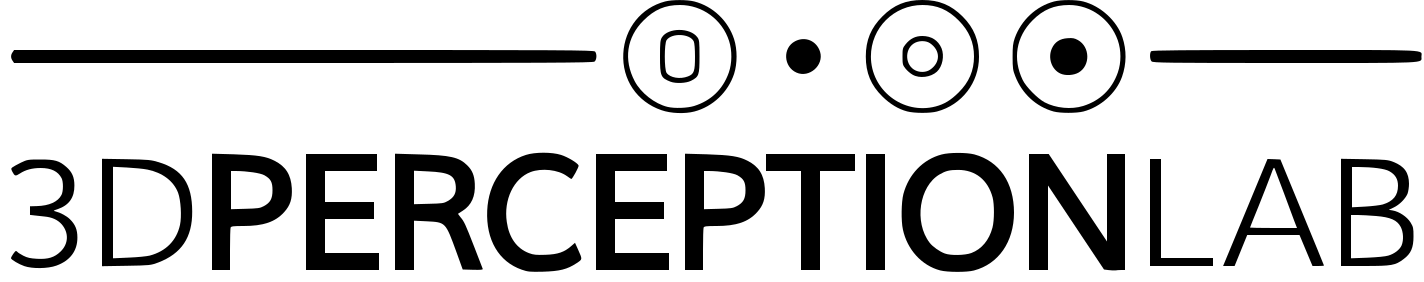
\includegraphics[height=0.7cm]{images/3dpl}
  \end{center}
\end{minipage}
}

% Clear the navigation bar
\setbeamertemplate{navigation symbols}{}
 
\subject{Sujet de la présentation}

\begin{document}

\begin{frame}
\titlepage
\end{frame}

\begin{frame}
  \frametitle{Table of Contents}
  \small
  \tableofcontents
  \normalsize
\end{frame}

\section{Introduction}
\label{sec:partie1}

\begin{frame}
  \frametitle{Introduction}
  \begin{center}
  	A visually realistic, flexible and robust grasping system for real-time interaction in Virtual Reality environments
  \end{center}
  	
  \begin{figure}
  	\centering
  	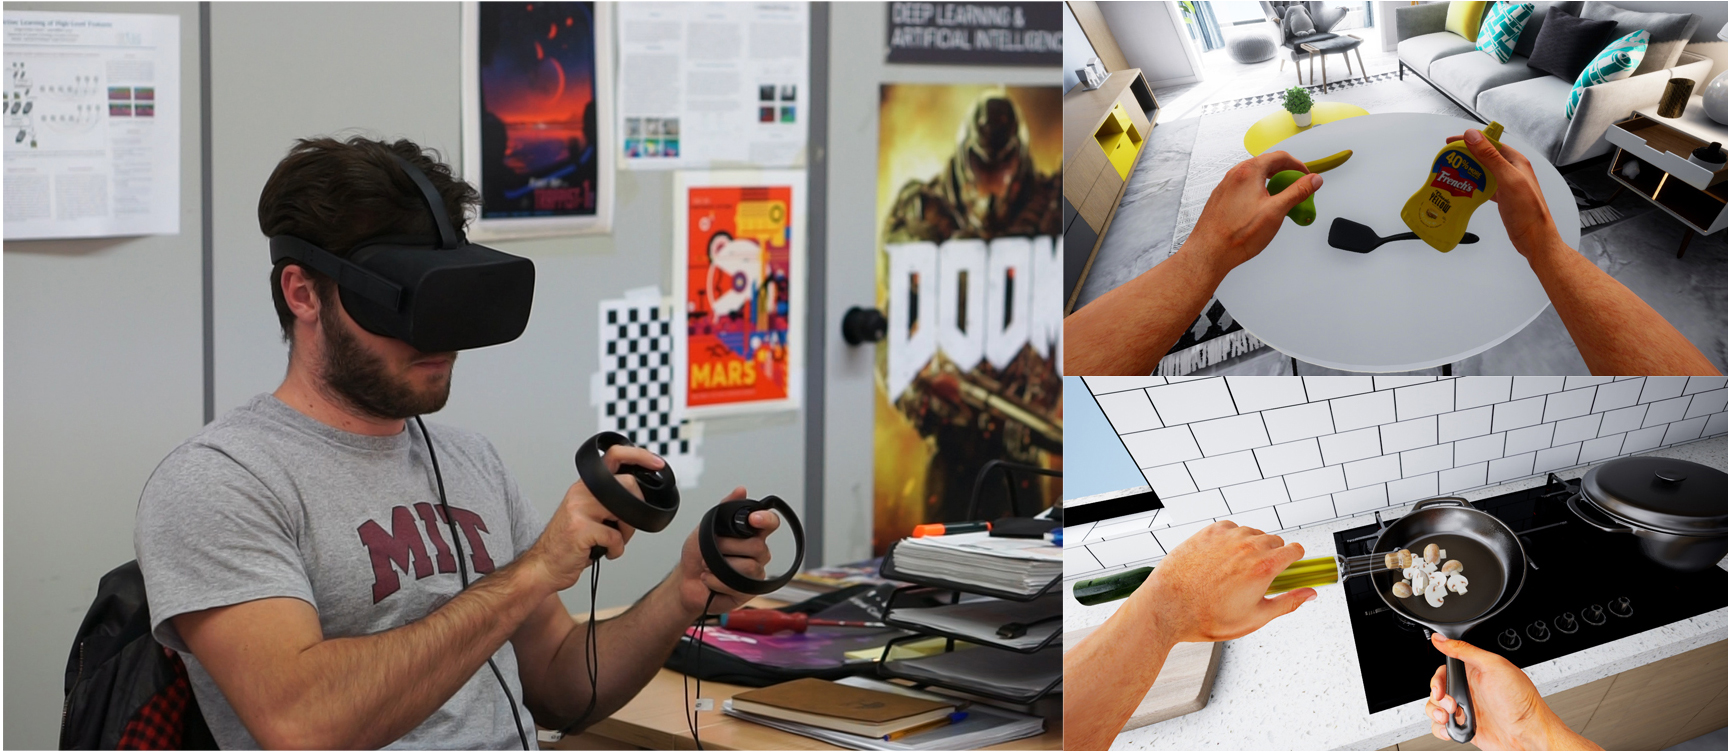
\includegraphics[width=0.9\textwidth]{images/intro}
  \end{figure}
\end{frame}

\begin{frame}
\frametitle{Introduction}
	\begin{itemize}
		\item VR objects extracted from the YCB dataset \cite{Calli2017}.
		\item Hands are controlled using handheld devices (e.g. Oculus Touch).
		\item Qualitative analysis: 
		\begin{itemize}
			\item motor control.
			\item finger movement realism.
			\item interaction realism.
		\end{itemize}
		\item Quantitative analysis:
		\begin{itemize}
			\item novel metric quantifying hand-object overlapping.
			\item time needed to grasp each object.
		\end{itemize}
	\end{itemize}
\end{frame}

\section{Motivation}

\begin{frame}
\frametitle{Motivation}
\begin{itemize}
	\item Currently existing interactions in VR applications lack of realism.
	\begin{itemize}
		\item Distance-based grasping.
		\item Predefined grasp animations.
	\end{itemize}
	\item Lack of open-source approaches.
	\item Extract data from visually realistic interactions with everyday objects.
\end{itemize}

\begin{figure}
	\centering
	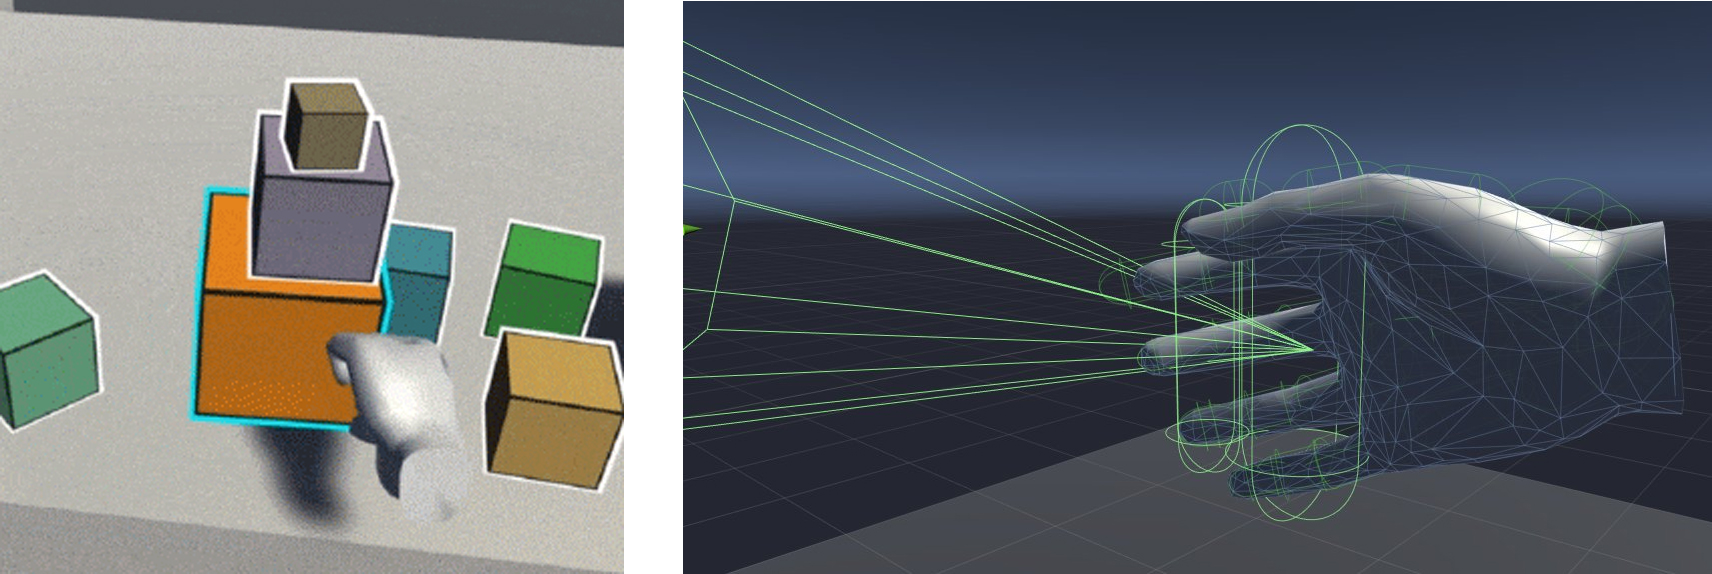
\includegraphics[width=0.7\textwidth]{images/grab}
	\caption{Distance grab example from Oculus Sample Framework \cite{oculusGrab}}
\end{figure}
\end{frame}


\section{Grasping System}

\begin{frame}
\frametitle{Grasping System}
The essence of our grasping system is how the hand is automatically fitted to the object shape. For this we needed to:
\begin{itemize}
	\item Configure the virtual hand:
	\begin{itemize}
		\item Choose the grasp animation according to a grasp taxonomy proposed by Feix et al. \cite{feix}.
		\item Experimentally place the capsule triggers on the phalanges.
	\end{itemize}
	\item Design and implement the grasping pipeline.
\end{itemize}
\end{frame}


\begin{frame}
\frametitle{Grasping System- hand configuration}

\textbf{Choose the grasp animation}

\begin{itemize}
	\item We analyzed 33 different grasp types from the taxonomy.
	\item The cylindrical grasp:
	\begin{itemize}
		\item Power grasp.
		\item Palm opposition.
	\end{itemize}
\end{itemize}

\begin{figure}
	\centering
	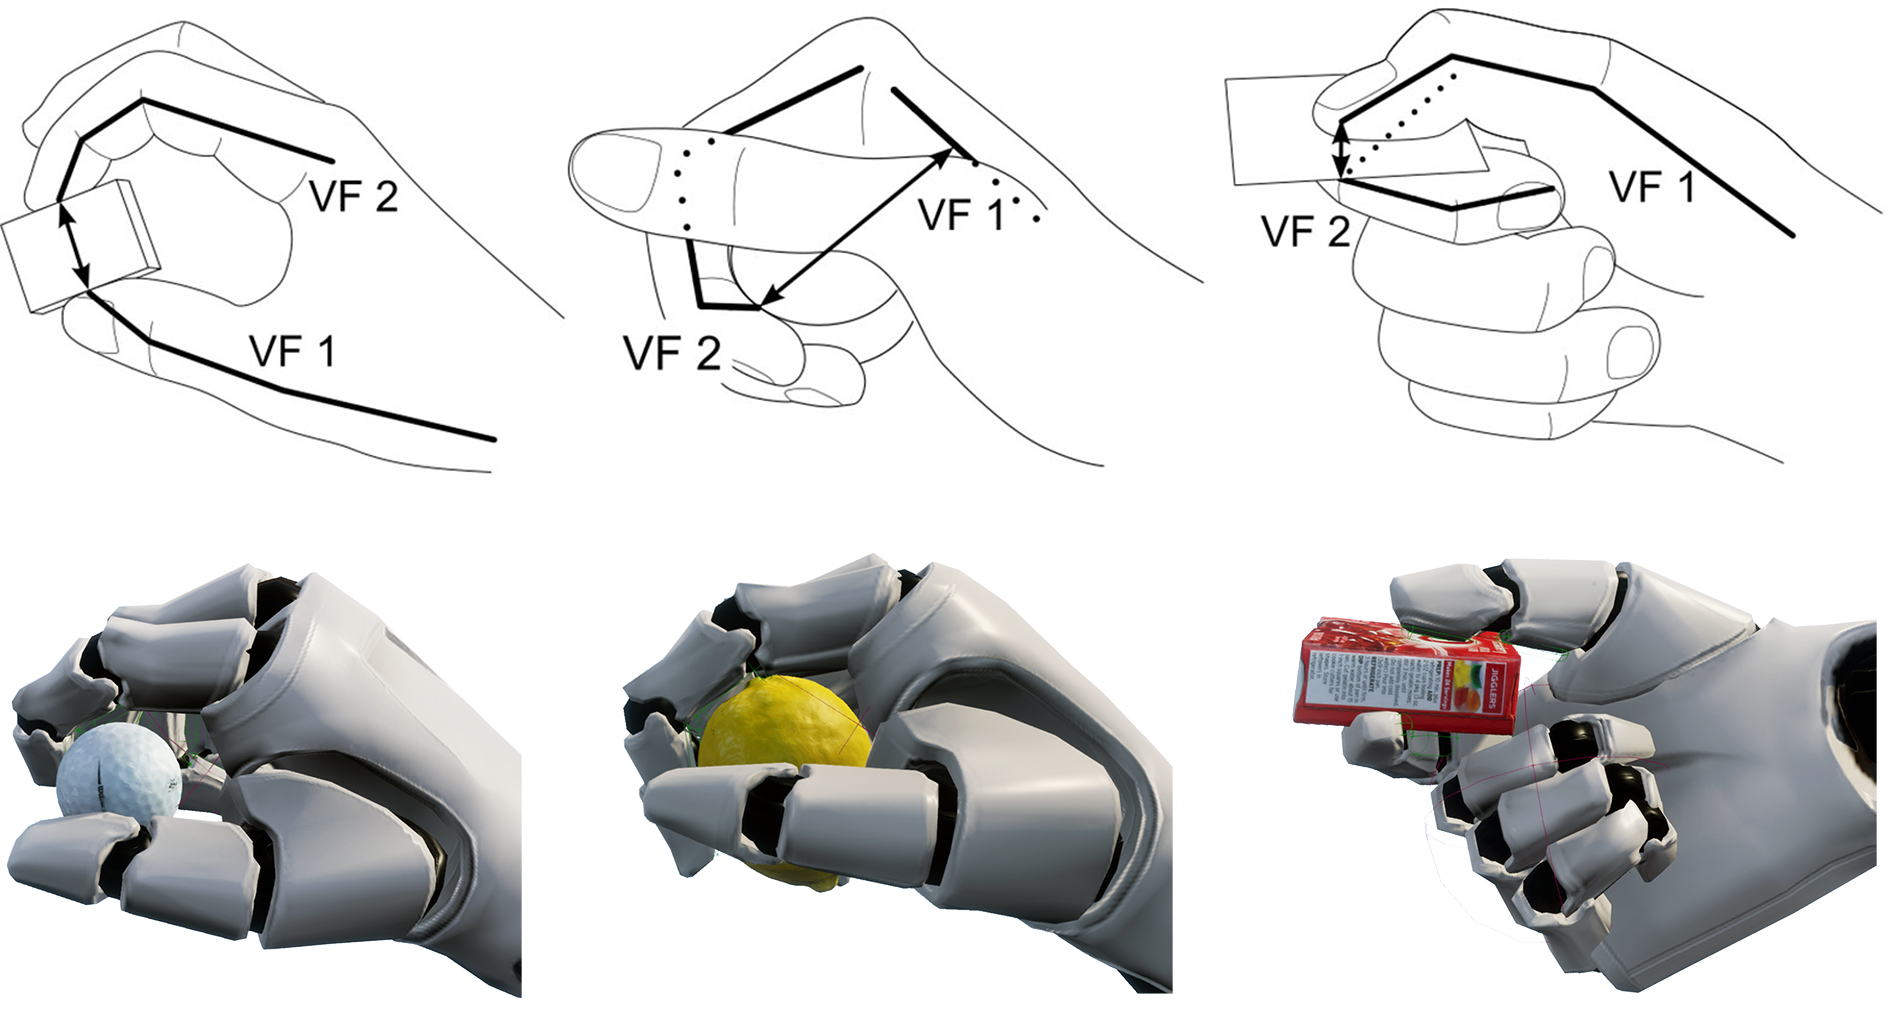
\includegraphics[width=0.6\textwidth]{images/grasp_taxonomy}
	\caption{From left to right: pad, palm and side opposition.}
\end{figure}
\end{frame}


\begin{frame}
\frametitle{Grasping System- hand configuration}

\textbf{Triggers placement}

\begin{itemize}
	\item Progressively increase the number of capsules to maintain performance.
	\item Interact with small and different shaped objects using capsules only on the distal phalanges.
	\begin{itemize}
		\item Slippery behavior because of the collision with middle phalanges.
		\item \textbf{Solution:} put capsule triggers on the middle phalanges.
	\end{itemize}
	\item Put a sphere trigger on the hand palm to enable palm opposition.
\end{itemize}

\begin{figure}
	\centering
	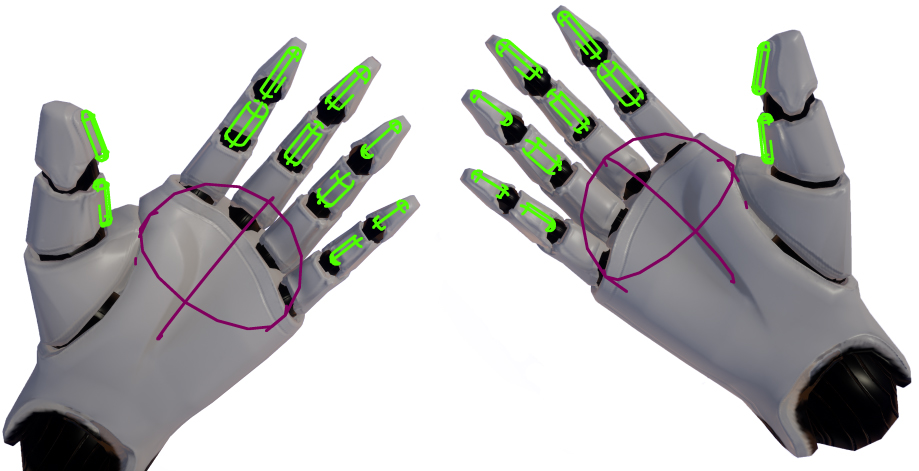
\includegraphics[width=0.5\textwidth]{images/mannequin_hands}
	\caption{In green, capsule triggers of the middle and distal phalanges. In purple, sphere triggers used to detect the nearest object the the hand palm.}
\end{figure}
\end{frame}


\begin{frame}
\frametitle{Grasping System- pipeline}

\definecolor{lightgreen}{RGB}{166,196,138}
\definecolor{lightblue}{RGB}{143,184,237}

\tikzstyle{block} = [rectangle, draw, fill=lightgreen, 
text width=5em, text centered, rounded corners, minimum height=3em]
\tikzstyle{cloud} = [draw, ellipse, text centered, fill=lightblue, text width=4em,
minimum height=2em]
\tikzstyle{line} = [draw, -latex']

\begin{figure}[!t]
	\centering
	\resizebox{0.9\linewidth}{!}{
		\begin{tikzpicture}[node distance = 3cm, auto]
		% Place nodes
		\node [block] (init) {Object selection};
		\node [block, right of= init] (manager) {Interaction manager};
		\node [block, right of= manager] (movement) {Finger movement};
		\node [block, right of= movement] (logic) {Grasping logic};
		
		% Draw edges
		\path [line] (init) -- (manager);
		\path [line] (manager) -- (movement);
		\path [line] (movement) -- (logic);
		\end{tikzpicture}}$  $
	\label{fig:pipeline}
\end{figure}

\begin{itemize}
	\item Object selection
	\item Interaction manager
	\item Finger movement
	\item Grasping logic
\end{itemize}

\end{frame}


\begin{frame}
\frametitle{Grasping System- pipeline}

\textbf{Grasping logic}

\begin{equation} \label{eq:3}
f(th_{ph}, in_{ph}, mi_{ph}, palm)= 
\begin{cases}
true, & \text{if } (th_{ph} \lor palm) \\
& \land (in_{ph} \lor mi_{ph})\\
false,              & \text{otherwise}
\end{cases}
\end{equation}, where $th_{ph}$, $in_{ph}$, and $mi_{ph}$ are defined as

\begin{equation} \label{eq:4}
\begin{array}{l}
th_{ph} = thumb_{mid} \lor thumb_{dist} \\
in_{ph} = index_{mid} \lor index_{dist} \\
mi_{ph} = middle_{mid} \lor middle_{dist} \\
\end{array}
\end{equation}

\end{frame}


\section{Performance analysis}

\begin{frame}
\frametitle{Performance analysis}

\end{frame}


\begin{frame}
\frametitle{Performance analysis- qualitative}

\end{frame}

\begin{frame}
\frametitle{Performance analysis- quantitative}

\begin{figure}
	\centering
	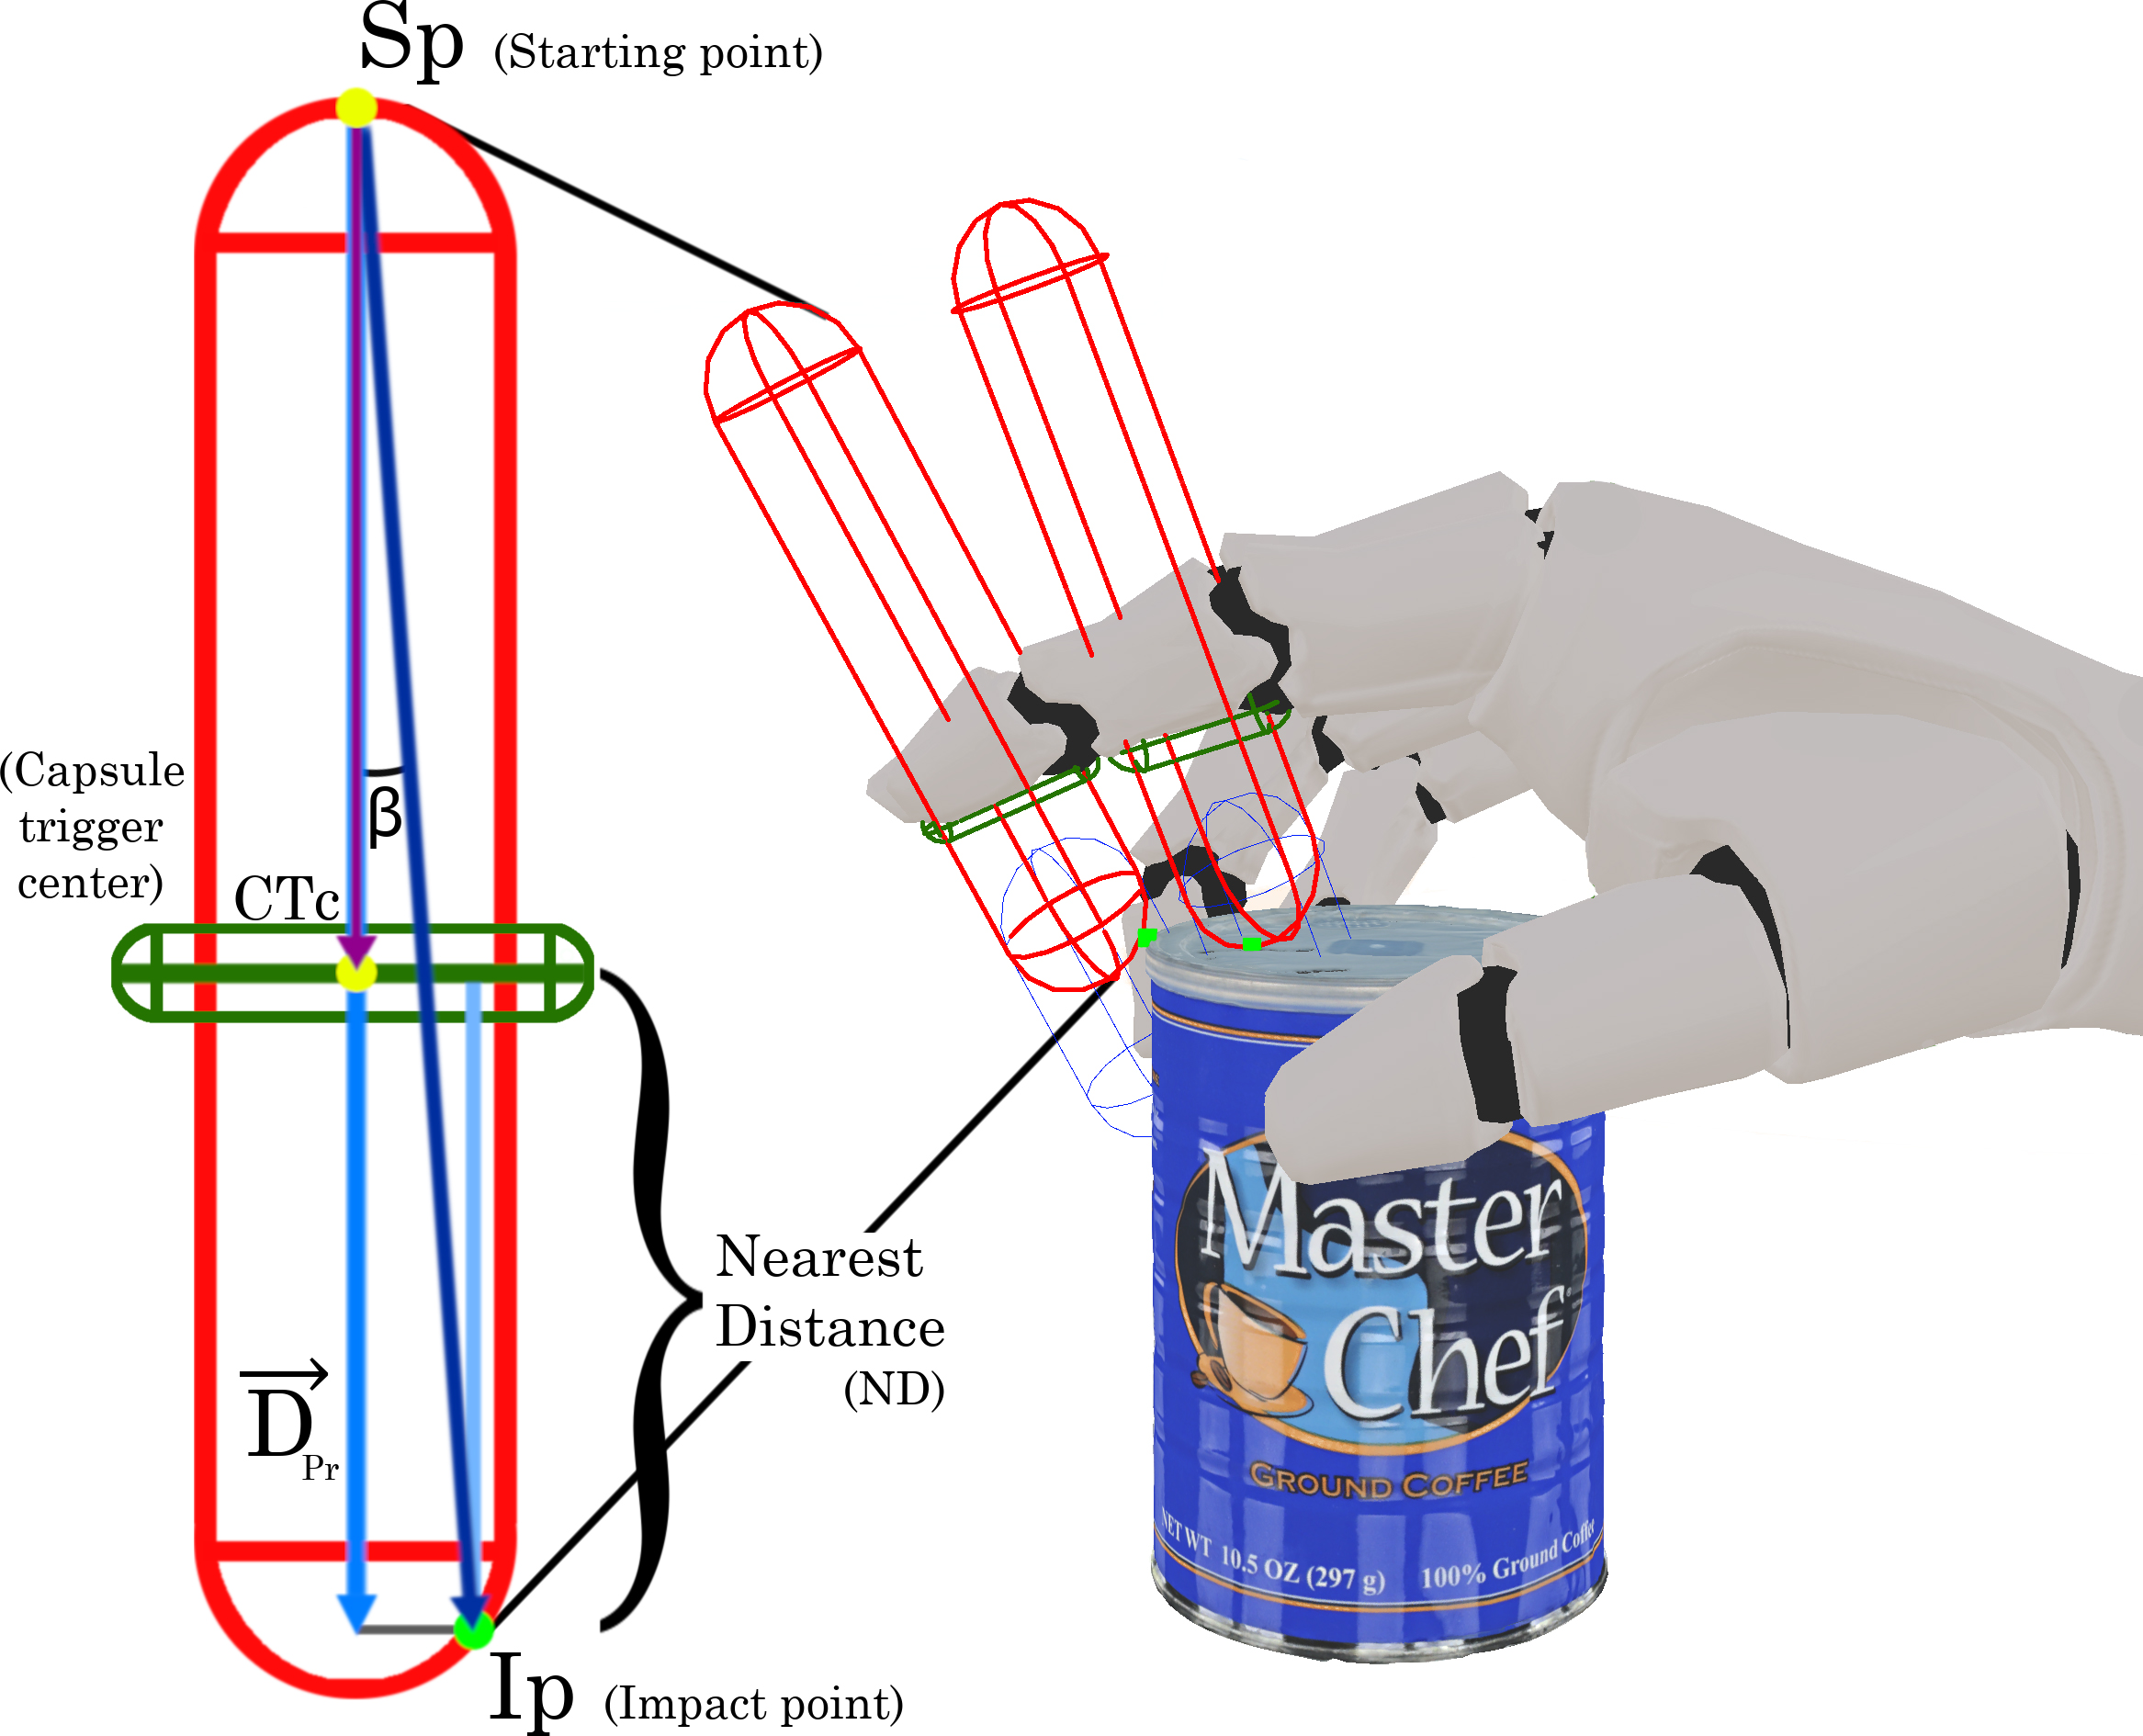
\includegraphics[width=0.7\textwidth]{images/distanceCalculusMod}
\end{figure}

\end{frame}


\begin{frame}
\frametitle{Performance analysis- procedure}

\end{frame}

\section{Results}

\begin{frame}
\frametitle{Results}

\end{frame}

\begin{frame}
\frametitle{Results- qualitative}

\end{frame}

\begin{frame}
\frametitle{Results- quantitative}

\begin{figure}
	\centering
	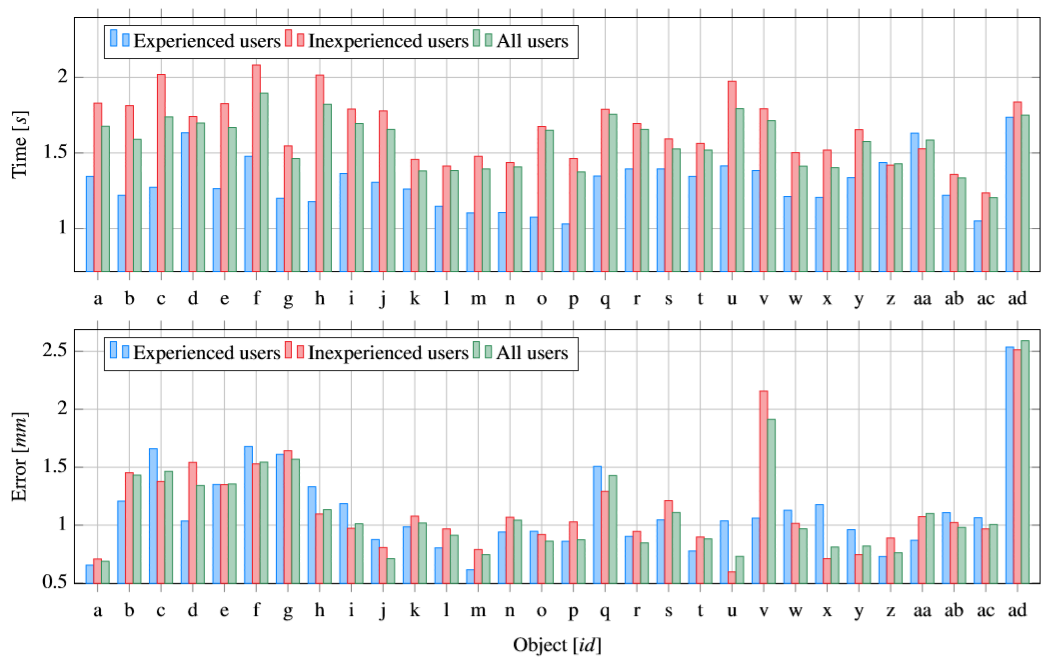
\includegraphics[width=0.9\textwidth]{images/results}
	\caption{Average time (top) needed to grasp each object and average error (bottom) of the performed grasps.}
\end{figure}

\end{frame}

\section{In Summary}



\begin{frame}
  \frametitle{Questions}
  \begin{center}
    Merci pour votre attention.

    Avez-vous des questions ?
  \end{center}
\end{frame}

\newcounter{lastframe}
\setcounter{lastframe}{\insertframenumber}

\begin{frame}[allowframebreaks]{References}
\bibliographystyle{authoryear-fr}
\bibliography{references}
\end{frame}

\setcounter{framenumber}{\thelastframe}

\end{document}
